\documentclass[12pt,a4paper]{report}
%adjust your page margins here
\usepackage[top=15mm, bottom=22mm, left=30mm,right=20mm]{geometry} % setting the page alignment with this package
\usepackage[pdftex]{graphicx} %for embedding images
\usepackage[%dvips, % commented for pdflatex
bookmarks,  colorlinks=false]{hyperref} %for creating links in the pdf version and other additional pdf attributes, no effect on the printed document
\hypersetup{%
    pdfborder = {0 0 0}
}
\usepackage[final]{pdfpages} %for embedding another pdf, remove if not required
\usepackage{float} %used for figure placement with H as a parameter
\usepackage{hyperref}
\usepackage{pslatex} % for times new roman, old package, but works
\usepackage{array} % for making text bold in table
\usepackage{setspace}
\usepackage{float}
\usepackage{enumerate} % list numbering
\usepackage{longtable} % making tables that runs across pages
\usepackage{ragged2e}  % package for text justification
\usepackage{amsmath}  % package for maths 
\usepackage{makeidx} % package for making index  
\usepackage{showidx} % print index
\usepackage[font=small,labelfont=bf]{caption}
\usepackage[utf8]{inputenc}
\makeindex
\def\figurename{\textbf{Figure }}

\usepackage{listings}
\usepackage{color}

\definecolor{dkgreen}{rgb}{0,0.6,0}
\definecolor{gray}{rgb}{0.5,0.5,0.5}
\definecolor{mauve}{rgb}{0.58,0,0.82}
 
\lstset{ %
  language=Java,                % the language of the code
  basicstyle=\footnotesize,           % the size of the fonts that are used for the code
  numbers=left,                   % where to put the line-numbers
  numberstyle=\tiny\color{gray},  % the style that is used for the line-numbers
  stepnumber=1,                   % each line is numbered
  numbersep=5pt,                  % how far the line-numbers are from the code
  backgroundcolor=\color{white},      % choose the background color. You must add \usepackage{color}
  showspaces=false,               % show spaces adding particular underscores
  showstringspaces=false,         % underline spaces within strings
  showtabs=false,                 % show tabs within strings adding particular underscores
  frame=single,                   % adds a frame around the code
  rulecolor=\color{black},        % if not set, the frame-color may be changed on line-breaks within not-black text (e.g. commens (green here))
  tabsize=2,                      % sets default tabsize to 2 spaces
  captionpos=b,                   % sets the caption-position to bottom
  breaklines=true,                % sets automatic line breaking
  breakatwhitespace=false,        % sets if automatic breaks should only happen at whitespace
  title=\lstname,                   % show the filename of files included with \lstinputlisting;
                                  % also try caption instead of title
  keywordstyle=\color{blue},          % keyword style
  commentstyle=\color{dkgreen},       % comment style
  stringstyle=\color{mauve},         % string literal style
  escapeinside={\%*}{*)},            % if you want to add a comment within your code
  morekeywords={*,...}               % if you want to add more keywords to the set
}

%For the header and footer
\usepackage{fancyhdr}
\fancypagestyle{plain}{%
\fancyfoot[L]{\emph{Department of Information Technology, DBIT, Mumbai}} % except the center
\fancyfoot[R]{\thepage}
\renewcommand{\headrulewidth}{0.4pt}
\renewcommand{\footrulewidth}{0.4pt}
}

\pagestyle{fancy}

%\rhead{\emph{NAME OF PROJECT}}

\fancyfoot[LO,LE]{\emph{Department of Information Technology, DBIT, Mumbai}}
\cfoot{}
\fancyfoot[RO, RE]{\thepage}
\renewcommand{\headrulewidth}{0.4pt}
\renewcommand{\footrulewidth}{0.4pt}
%For the header and footer Over

%Page Border
\usepackage{pgf}
\usepackage{pgfpages}

\pgfpagesdeclarelayout{boxed}
{
  \edef\pgfpageoptionborder{0pt}
}
{
  \pgfpagesphysicalpageoptions
  {%
    logical pages=1,%
  }
  \pgfpageslogicalpageoptions{1}
  {
    border code=\pgfsetlinewidth{2pt}\pgfstroke,%
    border shrink=\pgfpageoptionborder,%
    resized width=.95\pgfphysicalwidth,%
    resized height=.95\pgfphysicalheight,%
    center=\pgfpoint{.5\pgfphysicalwidth}{.5\pgfphysicalheight}%
  }%
}
\pgfpagesuselayout{boxed}
\setlength{\parindent}{1cm}
%GLOBAL SETTINGS OVER, DOCUMENT BEGINS
\begin{document}
\renewcommand\bibname{References}
\lhead{ }

%FROM HERE YOUR PAGES START GETTING ADDED
\newpage
\begin{center}
\thispagestyle{empty}
\LARGE{\textbf{Rubrics - A Student Evaluation System}}\\[0.1cm]
\vspace{0.5cm}
\Large{\textbf{\\Submitted in partial fulfillment of the requirements}}
\vspace{0.5cm}
\Large{\textbf{\\of the degree of}}
\vspace{0.5cm}
\LARGE{\textbf{\\Bachelor of Engineering}}
\vspace{0.5cm}
\Large{\textbf{\\by}}
\vspace{0.5cm}

\author[\textbf{Krupal Jadhav &&  27}\\

\vspace{0.5cm}
\Large{\textbf{Supervisor:}}\\
\vspace{0.5cm}
\Large{\textbf{Prof. Tayyabali Sayyad}}\\
\vspace{2cm}

\includegraphics[scale=1.6]{project/images/uop-logo.jpg}\\
\vspace{1cm}
\LARGE{\textbf{UNIVERSITY OF MUMBAI}}
\newpage
\end{center}
% includes the cover page
\newpage
\begin{center}
\thispagestyle{empty}
\LARGE{\textbf{Rubrics - A Student Evaluation System}}\\[0.1cm]
\vspace{0.1cm}
\Large{\textbf{\\Submitted in partial fulfillment of the requirements}}
\vspace{0.4cm}
\Large{\textbf{\\of the degree of}}
\vspace{0.4cm}
\LARGE{\textbf{\\Bachelor of Engineering}}
\vspace{0.4cm}
\Large{\textbf{\\by}}\\
\vspace{0.5cm}
\author[\textbf{Krupal Jadhav &&  27}\\
\vspace{0.4cm}
\Large{\textbf{Supervisor:}}\\
\vspace{0.4cm}
\Large{\textbf{Prof. Tayyabali Sayyad}}\\
\vspace{1cm}

\includegraphics[scale=0.32]{project/images/IMG-20170422-WA0009}\\
\vspace{0.4cm}
\Large{\textbf{Department of Information Technology}}\\
\vspace{0.4cm}
\Large{\textbf{Don Bosco Institute of Technology}}\\
%\large{\textbf{Vidyavihar Station Road, Mumbai - 400070}}
\large{\textbf{\\2016-2017}}\\
\vspace{1cm}
\Large{\textbf{AFFILIATED TO\\}}
\vspace{0.4cm}
\LARGE{\textbf{UNIVERSITY OF MUMBAI}}
\newpage
\end{center}
\newpage

%\newpage
\begin{center}
\thispagestyle{empty}
\Large{\textbf{A PROJECT REPORT\\ON}}\\[0.3cm]
\Large{\textsc {\textbf{``NAME OF PROJECT''}}}\\
\Large{\textbf{\\Submitted to}}
\LARGE{\textbf{\\UNIVERSITY OF MUMBAI\\}}
\large{\textbf{\\In Partial Fulfilment of the Requirement for the Award of\\}}
\LARGE{\textbf{\\BACHELOR'S DEGREE IN\\INFORMATION TECHNOLOGY}}
\vspace{0.3cm}
\Large{\textbf{\\BY}}\\[0.3cm]
\begin{table}[h]
\centering
\Large{
\begin{tabular}{>{\bfseries}lc>{\bfseries}r}
GROUP MEMBER A & & ROLL NUMBER A\\GROUP MEMBER B & & ROLL NUMBER B\\GROUP MEMBER C & & ROLL NUMBER C\\GROUP MEMBER D & & ROLL NUMBER D\\
\end{tabular}}
\end{table}
\large{\textbf{UNDER THE GUIDANCE OF}}\\
\large{\textbf{PROF. GUIDE NAME}}\\[0.5cm]

\includegraphics[scale=0.5]{project/images/jscoe_logo}\\
\large{\textbf{DEPARTMENT OF INFORMATION TECHNOLOGY}}\\
\Large{\textbf{NAME OF COLLEGE}}\\
\large{\textbf{LOCATION IN MUMBAI, MUMBAI - PINCODE}}
\large{\textbf{\\2012-2013}}\\[0.5cm]
\Large{\textbf{AFFILIATED TO}}\\[0.5cm]

\includegraphics[scale=1.0]{project/images/uop-logo}\\
\LARGE{\textbf{UNIVERSITY OF MUMBAI}}
\newpage

\end{center}
%\newpage


% includes the certificate page
\begin{center}
\thispagestyle{empty}

\LARGE{\textbf{DON BOSCO INSTITUTE OF TECHNOLOGY}} \\ 
\large{\textbf{Vidyavihar Station Road, Mumbai - 400070}}\\[0.5cm]
\Large{\textbf{Department of Information Technology}}\\[1.5cm]

%
\includegraphics[scale=0.5]{project/images/jscoe_logo}\\[0.5cm]

{\Huge \textbf{CERTIFICATE}}\\[0.5cm]
\end{center}
\linespread{1.13}

\large{\justify{This is to certify that the project entitled }\textbf{\Large{`Rubrics - A Student Evaluation System'}} is a bonafide  work of  \\

\begin{table}[h]
\centering
\large{
\begin{tabular}{>{\bfseries}lc>{\bfseries}r}
Deepesh Gupta & & 25\\Krupal Jadhav & & 27\\Kaustubh Kundu & & 34\\Sushant Yadav & & 66\\
\end{tabular}}
\end{table}

\justify submitted to the University of Mumbai in partial fulfillment of the requirement for the award of the degree of \textbf{\Large{Undergraduate}} in \textbf{\Large{Bachelor of Information Technology}} \\[0.25cm]
\large{\textbf{Date:\hspace*{1.0cm}/\hspace*{1.0cm}/}}\\
%\large{\textbf{Date:\date{}}}
\begin{spacing}{0}
\vspace{2.0cm}
\large{\textbf{Prof. Tayyabali Sayyad}}\hspace*{2.8in}\large{\textbf{}}\\
\hspace*{0.55in}\textbf{(Guide Name)}\hspace*{2.7in}\textbf{}\\[3cm]

\large{\textbf{Prof. Janhavi Baikerikar}}\hspace*{1.4in}\large{\textbf{Dr. Prasanna Nambiar}}\\
\hspace*{0.29in}\textbf{(HOD, IT Department)}\hspace*{2.1in}\textbf{(Principal)}\\[3cm]

%\hspace*{0.5cm}\large{\textbf{(Prof. HOD NAME)}}\hspace*{0.8in}\large{\textbf{(Dr. PRINCIPAL NAME)}}\\
%\textbf{HOD, Computer Department}\hspace*{0.8in}\textbf{Principal}\hspace*{1.1in}
\end{spacing} 
\newpage

% includes the Approval page
\begin{center}
\thispagestyle{empty}

\LARGE{\textbf{DON BOSCO INSTITUTE OF TECHNOLOGY}} \\ 
\large{\textbf{Vidyavihar Station Road, Mumbai - 400070}}\\[0.5cm]
\Large{\textbf{Department of Information Technology}}\\[1.5cm]

%
\includegraphics[scale=0.5]{project/images/jscoe_logo}\\[0.5cm]

{\Huge \textbf{Project Report Approval for B.E.}}\\[0.5cm]
\end{center}
\linespread{1.13}

\large{\justify{This project report entitled }\textbf{\Large{`Rubrics - A Student Evaluation System'}} by \textbf{\Large{Krupal Jadhav, Deepesh Gupta, Kaustubh Kundu, Sushant Yadav}} is approved for the degree of \textbf{\Large{Bachelor of Engineering in Information Technology}}
%\vspace{0.30cm}
\begin{flushright}
\Large{\textbf{(Examiner's Name and Signature)}}\\[1cm]
\hspace*{0.7in}\textbf{1. ---------------------------------------}\\[1cm]
\hspace*{0.7in}\textbf{2. ---------------------------------------}\\[2cm]
\Large{\textbf{(Supervisor's Name and Signature)}}\\[1cm]
\hspace*{0.7in}\textbf{1. ---------------------------------------}\\[1cm]
\Large{\textbf{( Chairman)}}\\[1cm]
%\vspace{0.25cm}
\hspace*{0.7in}\textbf{1. ---------------------------------------}\\[1cm]
\end{flushright}
\justify\large{\textbf{Date:}}\\
\justify\large{\textbf{Place: }} 
\newpage

% includes the 

\begin{center}
\thispagestyle{empty}

\LARGE{\textbf{DON BOSCO INSTITUTE OF TECHNOLOGY}} \\ 
\large{\textbf{Vidyavihar Station Road, Mumbai - 400070}}\\[0.5cm]
\Large{\textbf{Department of Information Technology}}\\[1.5cm]

%
\includegraphics[scale=0.5]{project/images/jscoe_logo}\\[0.5cm]

{\Huge \textbf{Declaration}}\\[0.5cm]
\end{center}
\linespread{1.13}

\large{\justify{I declare that this written submission represents my ideas in my own words and where others' ideas or words have been included, I have adequately cited and referenced the original sources. I also declare that I have adhered to all principles of academic honesty and integrity and have not misrepresented or fabricated or falsified any idea / data / fact / source in my submission. I understand that any violation of the above will be cause for disciplinary action by the Institute and can also evoke penal action from the sources which have thus not been properly cited or from whom proper permission has not been taken when needed. }

\begin{spacing}{0}
\vspace{3.0cm}
%\begin{justify}
\Large{\hfill\textbf{(----------------------------)}\\
\vspace{0.5cm}
\hspace{10.5cm}\textbf{Krupal Jadhav (27)}}\\
%\end{justify}
\end{spacing}
\justify\large{\textbf{Date:}}
 
\newpage

% includes the acknowledgements page
%\begin{center}
\thispagestyle{empty}
\LARGE{\textbf{Acknowledgements}}\\[1cm]
\end{center}
\linespread{1.13}
\large{\paragraph{}

This project was supported by Don Bosco Institute of Technology. We thank our teachers who provided insight and expertise that greatly assisted the project.\\
We thank Prof. Tayyabali Sayyad for assistance with forming the vision for our project.\\
We would also like to show our gratitude to the IT department teachers for sharing their pearls of wisdom with us during the course of this project. 



\begin{spacing}{0}
\vspace{3.0cm}
%\begin{justify}
\Large{\hfill\textbf{(----------------------------)}\\
\vspace{0.5cm}
\hspace{10.5cm}\textbf{Krupal Jadhav (27)}}\\
%\end{justify}
\end{spacing}
\justify\large{\textbf{Date:}}
 
%\newpage

\begin{center}
\thispagestyle{empty}
\vspace{2cm}
\LARGE{\textbf{Abstract}}\\[1.0cm]
\end{center}
\thispagestyle{empty}

\large{\paragraph{}
The online grading system has become very popular as everything is going to be digitalized. student evaluation System is designed to help evaluators, faculties to properly grade student work. viewing student work, managing rubrics and graphical analysis of student assignments related issues are made simple and easy.
}

\large{\paragraph{}
Rubrics evaluation system is the widespread practice in both the software industry and the educational institutes.This can make the system easier to navigate and to use maximizing the effectiveness of time and other resources.rubrics system allows the keeping of track of submissions and evaluated data in a form that can be easily accessed and analyzed in a consistent way.\\\\
\textbf{Keywords: }Rubrics, Document evaluation system % adds the Research Methodology page
\newpage

%TABLE OF CONTENTS AND LIST OF FIGURES ARE AUTOMATICALLY ADDED BY FOLLOWING COMMANDS
%ADD FIGURE OF TABLES IF YOU NEED TO, CHECK DOCUMENTATION
\pagenumbering{roman} %numbering before main content starts


%To reset the Header & Footer for TOC and LOF
\pagestyle{empty}
\addtocontents{toc}{\protect\thispagestyle{empty}}
\tableofcontents % adds Index Page
\vspace{0.1 mm}
\addtocontents{lof}{\protect\thispagestyle{empty}}
\listoffigures % adds List of Figures
\addtocontents{lot}{\protect\thispagestyle{empty}}
\listoftables % adds List of tables

%And reset back the settings we choose for Header and Footer
\pagestyle{fancy}

\newpage
\pagenumbering{arabic} %reset numbering to normal for the main content

\chapter{Introduction}
\section{Problem Statement}
To develop a software application that will help educators to grade students fairly based on rubrics. Rubrics are generally something that makes the life of an educator easier. Rather than adding an arbitrary grade to an assignment, with rubrics educators are able to determine exactly where a student’s work excelled beyond expectations and exactly where it lacked quality. Our software will provide a platform for the educators in which they would be able to create a grading rubric. The educator would define performance levels (like excellent, good, average, poor etc.) and parameters (like neatness, proper content etc.) for grading. Each performance level would have some weight assigned to it based on which
the software would calculate the student’s final score. This software will also provide a proper feedback to the students and will tell them what areas they need to work on based on their assignment submissions.\\
\section{Scope of the Project}\
Rubrics system provides a web-based and mobile-based platform to students as  well as the grader, where students can upload their work and the grader will evaluate their work according to the designed metric developed by the grader. This system displays all the performance of the student in a graphical format so that student will get the clear idea about where he/she is good or where he/she is lagging and what is pending jobs and what is completely done.Using Rubrics system, the grader can review the students work as well as give proper feedback to the student and get the personal attention from the grader.\\
\section{Current Scenario}
Currently there are four such student evaluation tools available online. The following table gives a brief list of their included features.
\begin {table}[H]
\begin{center}
\begin{tabular}{ | m{3.5cm} | m{2cm}| m{2cm}| m{2cm} |m{2.6cm}| m{2cm} | }
\hline
\textbf{Features} & \textbf{RubiStar} & \textbf{Moodle} & \textbf{iRubric} & \textbf{EssayTagger} & \textbf{Rubric System}\\ 
\hline
Multiple Templates & Yes & No & No & No & Yes\\
\hline
Dyanamic Create Templates & Yes & Yes & Yes & No & Yes\\
\hline
Graphical Performance Analysis & No & Yes & No & No & Yes\\
\hline
User Convenient & Yes & No & No & Yes & Yes\\
\hline
Pricing & Yes & Yes & Yes & Yes & No\\
\hline
Feeback to students & No & Yes & Yes & Yes & Yes\\
\hline
\end{tabular}\\
\caption {Current Scenario}
\end{center}
\end {table}


\section{Need for the Proposed System}
\begin{itemize}
\item To evaluate the quality of students.
\item To focus on measuring objectives(performance, behavior, and quality).
\item To develop a better way of communication between teachers and students.
\item To increase interest in ``performance-based education".
\end{itemize}
\section{Summary of the Results / Task completed }
\begin{itemize}
\item Developed a web-Prototype and Mobile Application Prototype
\item Did literature survey of various evaluation systems
\item Started Web and Android Application implementation(Coding)
\end{itemize}
\newpage

 % adds the introduction page
\chapter{Review of Literature }
\section{Literature Survey}
We have gone through various evaluation and grading tools as per our observation there are not single system which is been made for both android and website.The creation of rubrics system is very tedious and unclear to the user.The application are only targeted for certain events which is the biggest drawback.\\
There are hardly any feedback system that has been provided by this application system.Hence following is the summary that we have inferred from our research\\
\begin{figure}[H]
\centering
\hfill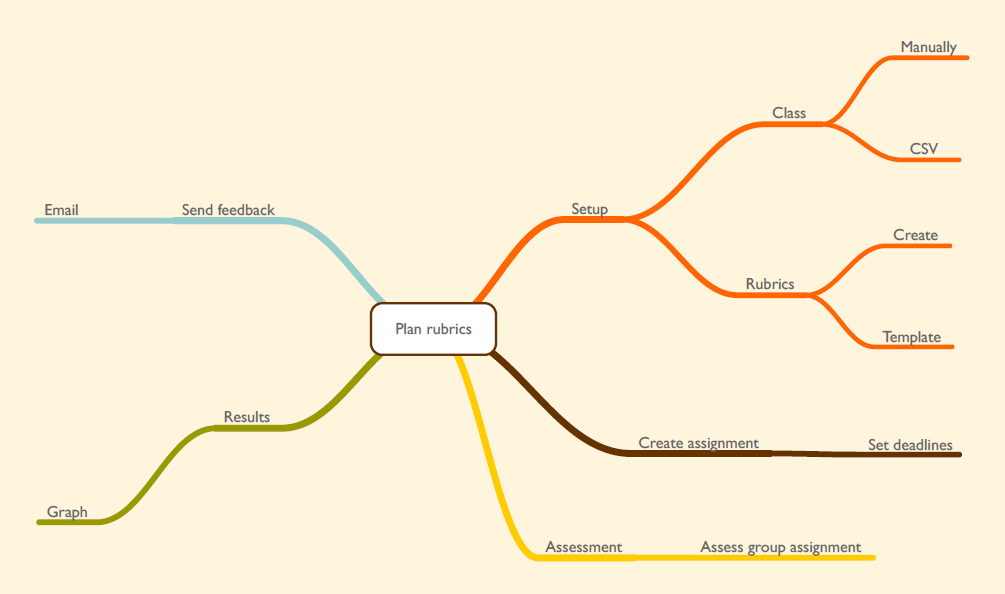
\includegraphics[scale=0.6]{project/images/mindmap}\hspace*{\fill}
\caption{Rubrics System}
\end{figure}
\newpage
{Comparison done between the tools / methods / algorithms}
\begin{table}[H]
\centering
\begin{tabular}{|l|l|l|l|l|l|}
\hline
\textbf{Features}                                                         & \textbf{Rubistar} & \textbf{Moodle} & \textbf{iRubrics} & \textbf{EssayTagger} & \textbf{Rubric System} \\ \hline
Multiple Template                                                         & Yes               & No              & No                & No                   & Yes                    \\ \hline
\begin{tabular}[c]{@{}l@{}}Dynamically create\\ template\end{tabular}     & Yes               & Yes             & Yes               & No                   & Yes                    \\ \hline
\begin{tabular}[c]{@{}l@{}}Graphical performance \\ analysis\end{tabular} & No                & Yes             & No                & No                   & Yes                    \\ \hline
User Convenient                                                           & Yes               & No              & No                & Yes                  & Yes                    \\ \hline
Cost                                                                      & Yes               & Yes             & Yes               & Yes                  & No                     \\ \hline
Feedback to student                                                       & No                & Yes             & Yes               & Yes                  & Yes                    \\ \hline
\end{tabular}
\caption{Comparison Between the tools}
\label{my-label}
\end{table} % adds the Literature Survey page
\chapter{Analysis and Design}
\section{Methodology / Procedure adopted}
We choose Extreme Programming (agile development) methodology for our project, Because this model Provides following Features:
\begin{itemize}
    \item Decrease the time required to avail some system features.
    \item Face to face communication and continuous inputs from customer representative leaves no space for guesswork.
    \item The end result is the high quality software in least possible time duration and satisfied customer.
\end{itemize}
We will conduct the weekly meetings with our project guide and do the project work/activities which will be assigned by guide and we will submit the weekly report to guide. We will maintain activity sheets from the beginning of the project work to track the activities which are planned, activities completed and carry forwarded.

\section{Analysis}
Based on the requirements gathered, how was the feasibility study of the project carried out?
The project is about the student evaluation system, so the study carried out on the comparison of the different student evaluation softwares.On comparison of different features of some softwares.the various system was referred for Evaluation system, which gives the idea of different ways of creating and evaluating students work.
If any requirements, were modified why they were modified?

\section{Proposed System}
Rubrics system provides a web-based and mobile-based platform to students as well as grader, where students can upload their work and the grader will evaluate their work according to the designed metric developed by grader.
This system displays all the performance of the student in a graphical format so that student will get the clear idea about where he/she is good or where he/she is lagging and what is pending jobs and what is completely done.
Using Rubrics system, grader can review the students work as well as give proper feedback to student and get the personal attention from grader.

\subsection{Advantages of the proposed system over existing systems}
\begin{enumerate}
    \item No Pricing.
    \item User-friendly system.
    \item Provides offline sync.
    \item Create dynamic templates.
    \item Graphical performance analysis.
    \item Interactive feedback to students.
    \item Multiple as well as built-in Templates.  
\end{enumerate}

\subsection{Development Hardware / Software requirements}

\textbf{Hardware requirements:}
\begin{itemize}
    \item Computer machine.
    \item Android Smartphone.
\end{itemize}
\textbf{Software requirements:}
\begin{itemize}
    \item Front End : Html, Css, JavaScript.
    \item Backend : SQLite, MySQL, PHP.
    \item Connectivity - PHP Wamp Server.
\end{itemize}
\textbf{Software tools:}
\begin{itemize}
    \item Android studio
    \item Text Editor
\end{itemize}

\textbf{Deployment Hardware / Software requirements}
\begin{enumerate}
\item Hardware required
    \begin{itemize}
        \item Computer
        \item Android smart-phone 
    \end{itemize}
 
\item Software required
    \begin{itemize}
        \item Web Browser        
        \item Android version 4.4 and above
    \end{itemize}
\end{enumerate}

\subsection{Design Details}

Different UML diagrams as per the project requirement (For e.g. Use Case Diagram)\\
\begin{figure}[!h]
\centering
\hfill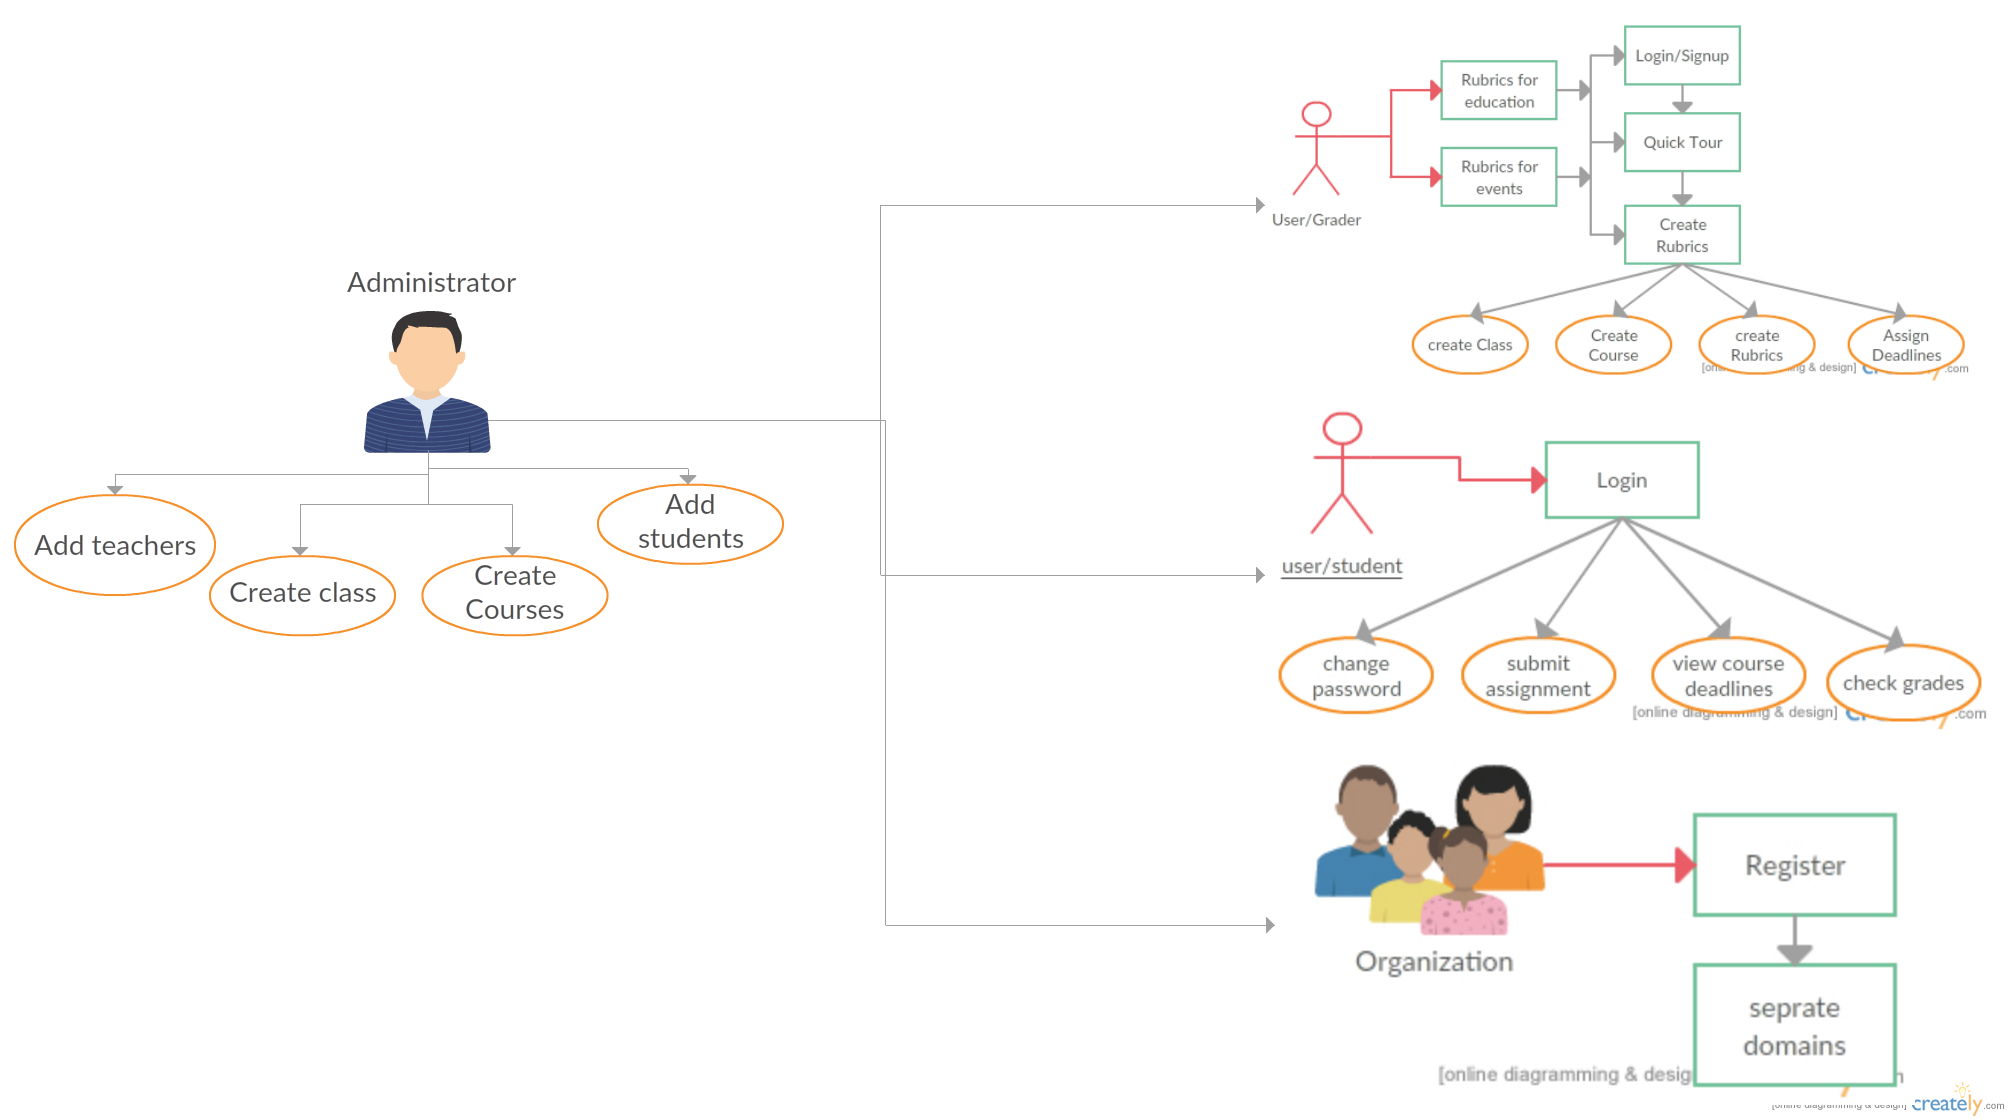
\includegraphics[scale=.22]{project/images/rubrics}\hspace*{\fill}
\caption{Connectivity diagram for Rubrics Student Evaluation System}
\end{figure}

In the above connectivity Diagram of rubrics student assessment tool admin, user and grader is there, they have to signup or login with their respective user ids and password.
\begin{itemize}
  \item After login the user will get a quick overview of system.grader have to logins into the system, the grader will get the interface of on which they can select that what type of rubrics they want to create like Rubric for education or Rubric for events.Then next step is to create rubrics for the selected type of event.After the rubric created the grader is done with their creating rubric/metrics, the student can submit their work for evaluation.When the grader did with the evaluation the student will be notified by mail.The job of the administrator is to add teachers, create the class, create courses and add students.
\end{itemize}

\subsection{Design details}
\begin{figure}[!h]

\hfill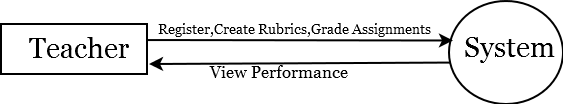
\includegraphics[scale=.65]{project/images/cfd}\hspace*{\fill}
\caption{Level 0 DFD diagram}
\end{figure}

\begin{figure}[!h]

\hfill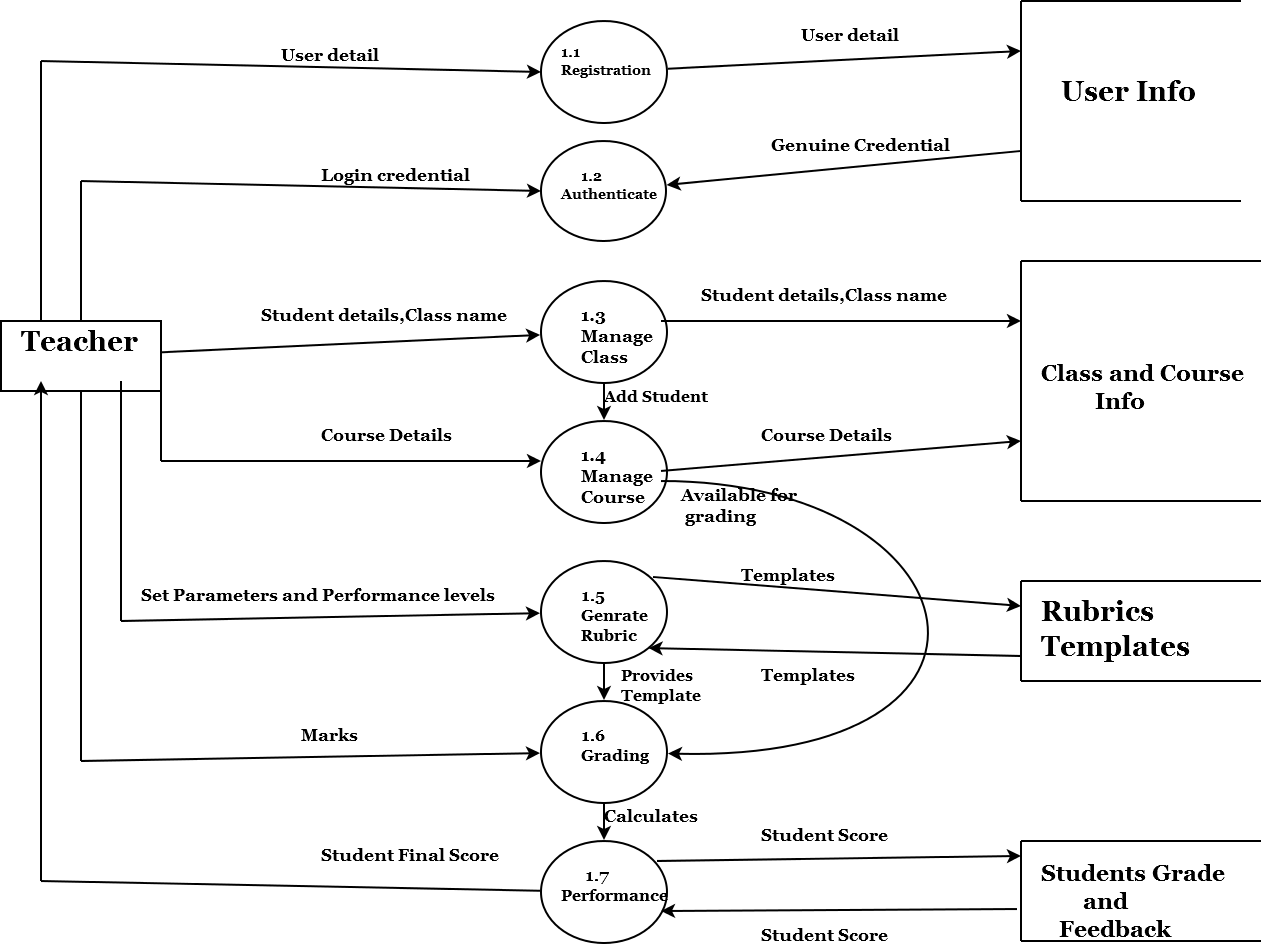
\includegraphics[scale=.37]{project/images/level1}\hspace*{\fill}
\caption{Level 1 DFD diagram}
\end{figure}

\chapter{Implementation}


\section{Implementation Plan \textit{for Sem – 8}}
Implementation Plan for the Sem - 8 to include the following:\\
Gantt chart
\begin{figure}[h]
	\centering
    \hfill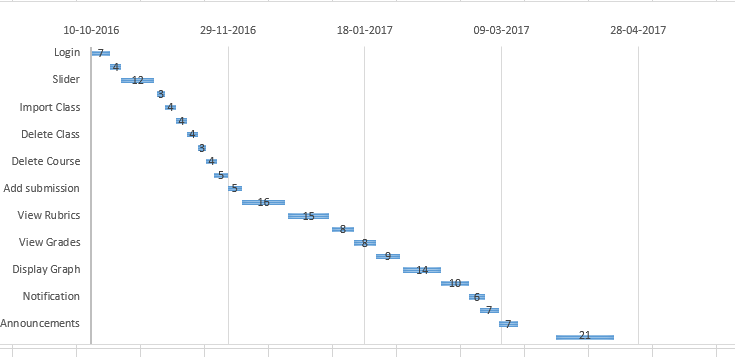
\includegraphics[scale=.85,angle=360]{project/images/Capture}\hspace{\fill}
    \caption{Gantt chart}
\end{figure}\\
\newpage
Work Break down structure \\ 
\begin{figure}[h]
	\centering
    \hfill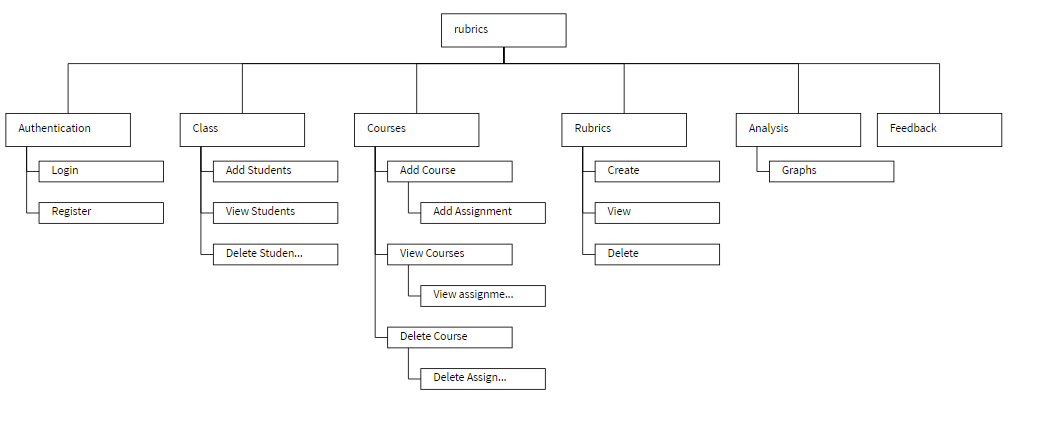
\includegraphics[scale=.60,angle=360]{project/images/wbs}\hspace{\fill}
    \caption{WBS chart}
\end{figure}\\

\section{Android and Web Application GUI}
\subsection{Android GUI}
\begin{figure}[!h]
\begin{minipage}[t]{0.5\linewidth}
    \centering
\hfill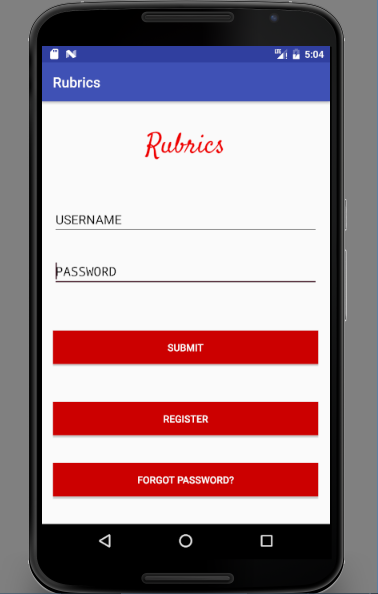
\includegraphics[scale=.65]{project/images/loginnew}\hspace*{\fill}
    \caption{Login Page}
    \label{f1}
\end{minipage}
\hspace{0.1cm}
\begin{minipage}[t]{0.5\linewidth} 
    \centering
\hfill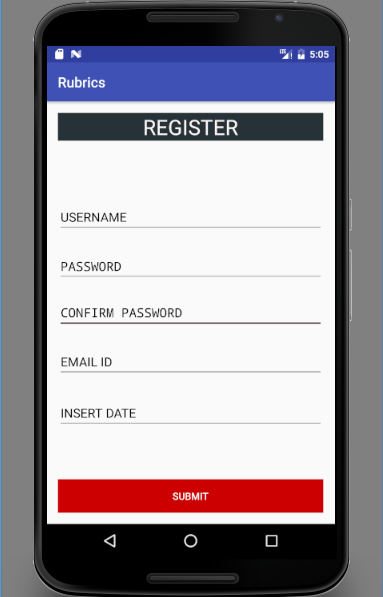
\includegraphics[scale=.65]{project/images/registernew}\hspace*{\fill}
    \caption{Registration Page}
    \label{f2}
\end{minipage}        
\end{figure}  

\begin{figure}[!h]
\begin{minipage}[t]{0.5\linewidth}
    \centering
\hfill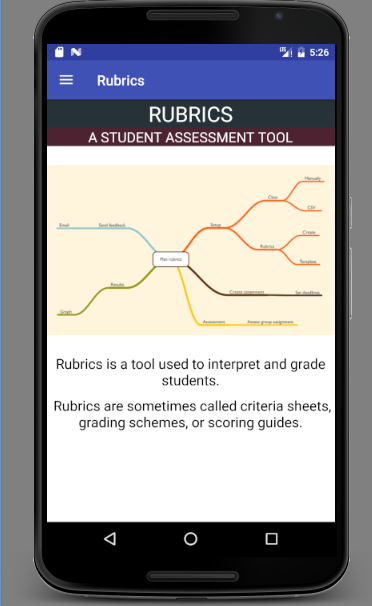
\includegraphics[scale=.65]{project/images/welcomepage}\hspace*{\fill}
    \caption{Quick Overview}
    \label{f1}
\end{minipage}
\hspace{0.1cm}
\begin{minipage}[t]{0.5\linewidth} 
    \centering
\hfill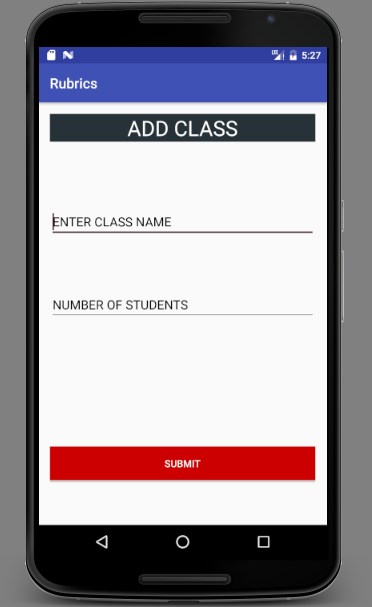
\includegraphics[scale=.65]{project/images/manageclassnew}\hspace*{\fill}
    \caption{Manage Class Page}
    \label{f2}
\end{minipage}        
\end{figure}  

\begin{figure}[!h]
\begin{minipage}[t]{0.5\linewidth}
    \centering
\hfill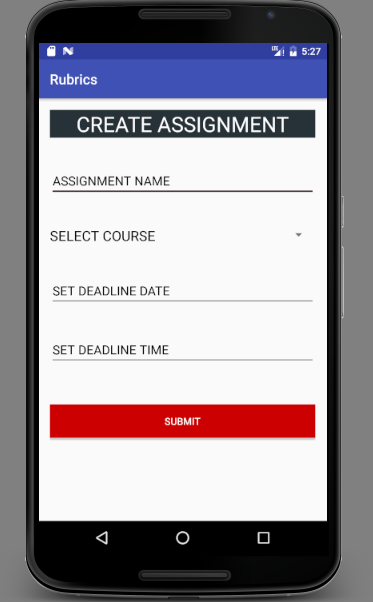
\includegraphics[scale=.65]{project/images/createassigmentnew}\hspace*{\fill}
    \caption{Create Asssignment}
    \label{f1}
\end{minipage}
\hspace{0.1cm}
\begin{minipage}[t]{0.5\linewidth} 
    \centering
\hfill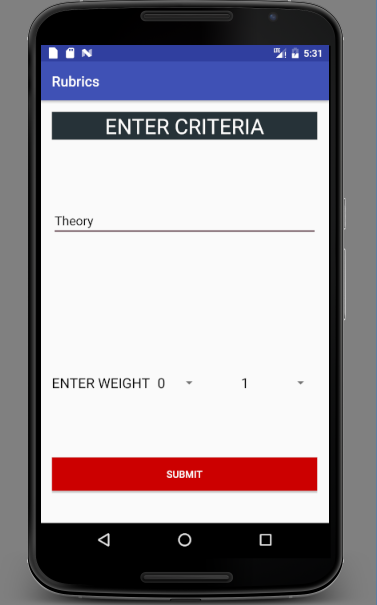
\includegraphics[scale=.65]{project/images/createrubricnew}\hspace*{\fill}
    \caption{Create Rubrics}
    \label{f2}
\end{minipage}        
\end{figure}  

\begin{figure}[!h]
\begin{minipage}[t]{0.5\linewidth}
    \centering
\hfill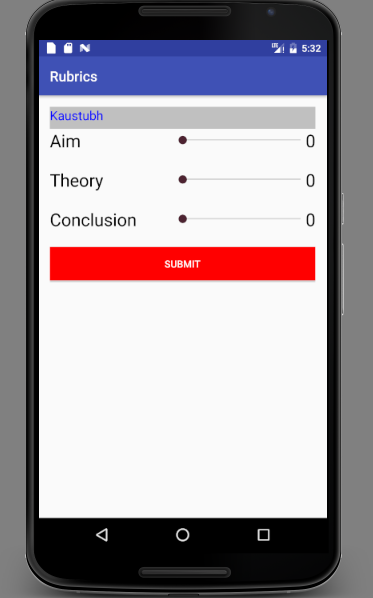
\includegraphics[scale=.65]{project/images/gradingnew}\hspace*{\fill}
    \caption{Start Grading}
    \label{f1}
\end{minipage}        
\end{figure}  

\subsection{Web GUI}
\begin{figure}[H]
\begin{minipage}[t]{0.5\linewidth}
    \centering
\hfill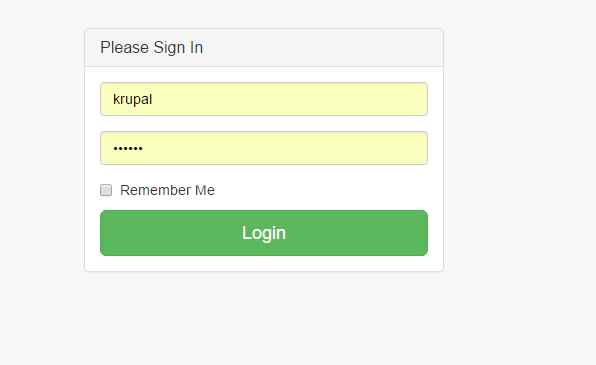
\includegraphics[scale=1]{project/11}\hspace*{\fill}
    \caption{Login}
    \label{f1}
\end{minipage}        
\end{figure}  

\begin{figure}[!h]
\begin{minipage}[t]{0.5\linewidth}
    \centering
\hfill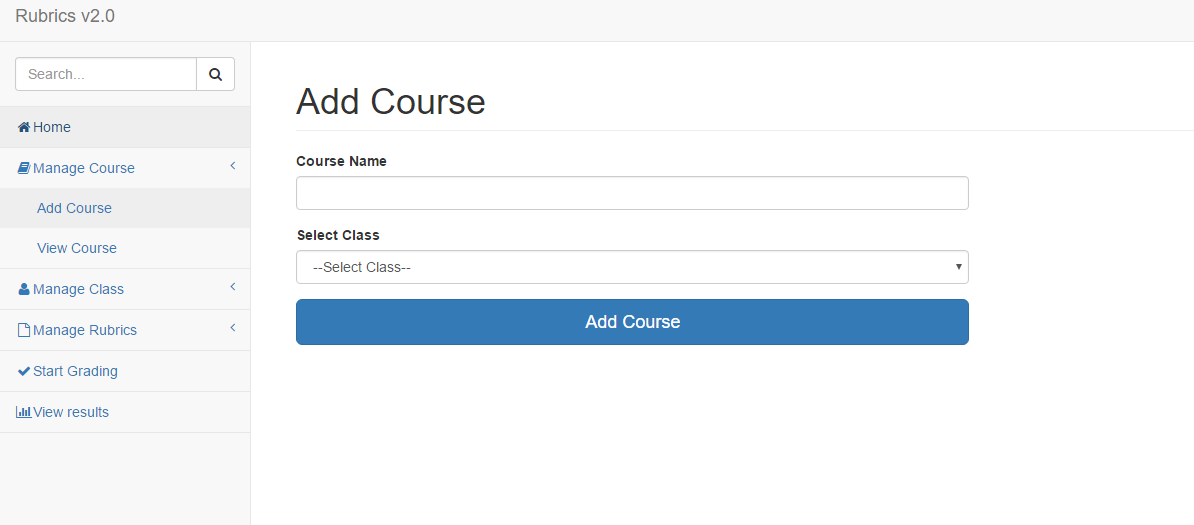
\includegraphics[width=17cm, height=11cm]{project/12}\hspace*{\fill}
    \caption{Add Course}
    \label{f1}
\end{minipage}        
\end{figure} 

\begin{figure}[!h]
\begin{minipage}[t]{0.5\linewidth}
    \centering
\hfill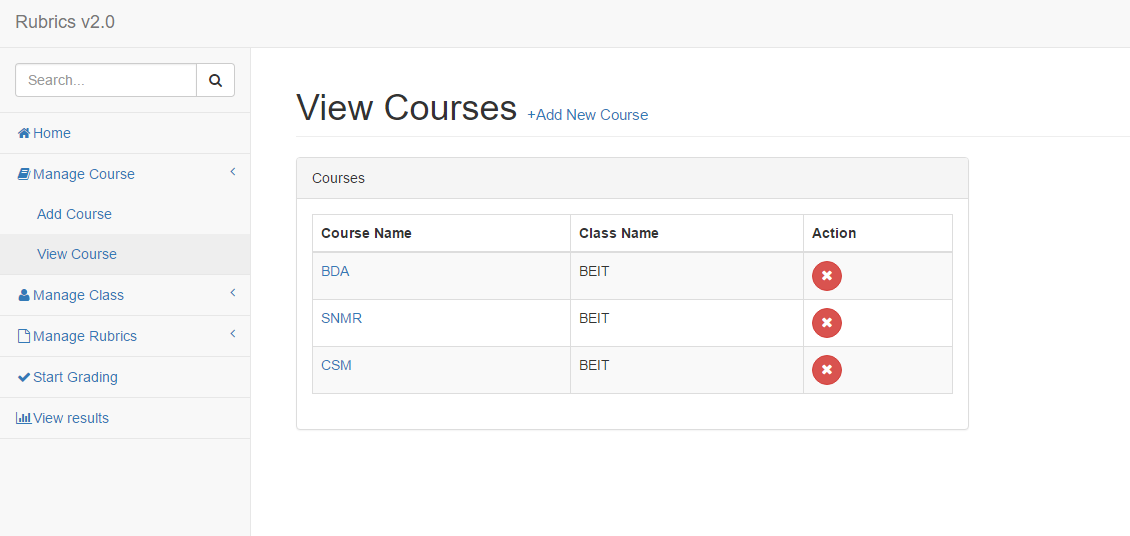
\includegraphics[width=17cm, height=11cm]{project/13}\hspace*{\fill}
    \caption{View Course}
    \label{f1}
\end{minipage}        
\end{figure}

\begin{figure}[!h]

\begin{minipage}[t]{0.5\linewidth}
    \centering
\hfill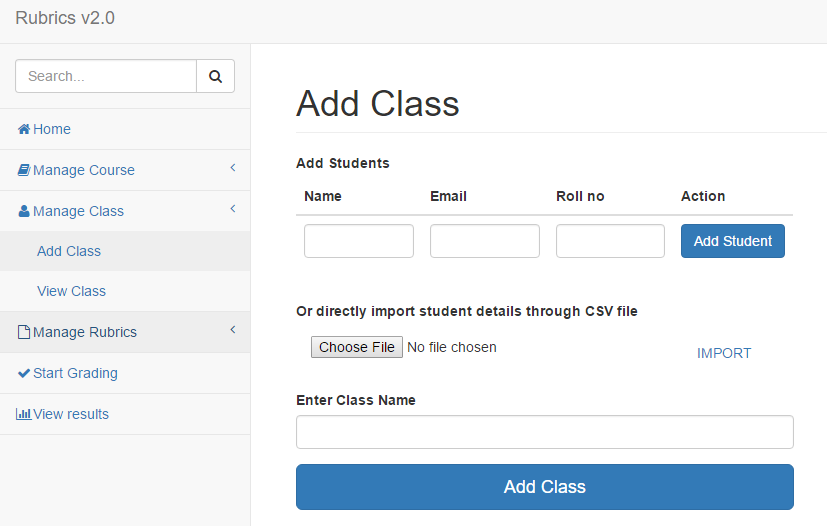
\includegraphics[width=17cm, height=12cm]{project/14}\hspace*{\fill}
    \caption{Add Class}
    \label{f1}
\end{minipage}        
\end{figure}

\begin{figure}[!h]
\begin{minipage}[t]{0.5\linewidth}
    \centering
\hfill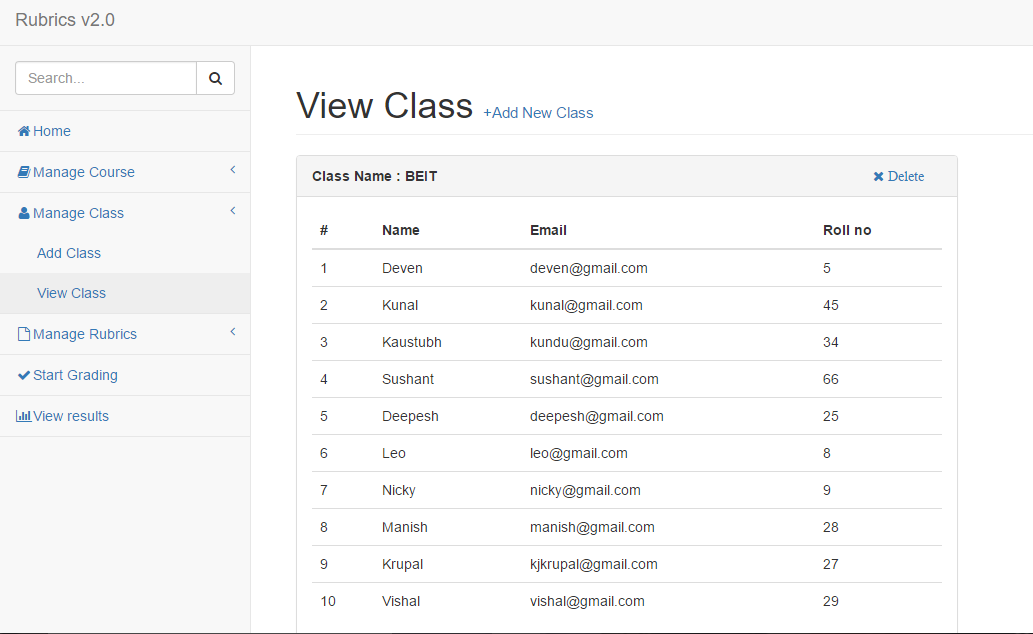
\includegraphics[width=17cm, height=11cm]{project/15}\hspace*{\fill}
    \caption{View Class}
    \label{f1}
\end{minipage}        
\end{figure}

\newpage

\section{Testing}
\vspace{-0.5cm}
Testing process constitutes checking errors in the code. The main objective of testing is to find the undiscovered errors in the code.\\
There are various methods of testing the code \\
\textbf{White Box Testing:}
To check the control structure of the program White box Testing can be used.
Test cases ensure that all the nationalities of the software have been tested at least once.\\
\textbf{Black Box Testing:}
Black box testing is designed to check if the software validations are properly done without considering the internal working of the software.\\
\textbf{Unit Testing:}
In Unit testing all the modules of the software are tested to check if they are in accordance with the modules provided during the design phase. Testing the internal logic of the code is the main motive of Unit testing. White box testing techniques are utilized to check if the control structure is good and does maximum error detection.

\subsection{Test Cases}
Test cases for Modules / component \\
\begin{figure}[H]
\centering
\hfill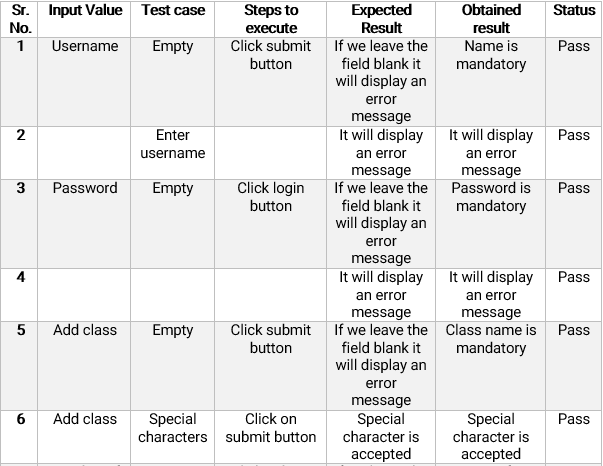
\includegraphics[scale=0.9]{project/images/test1}\hspace*{\fill}
\caption{Test case 1}
\end{figure}

\begin{figure}[H]
\centering
\hfill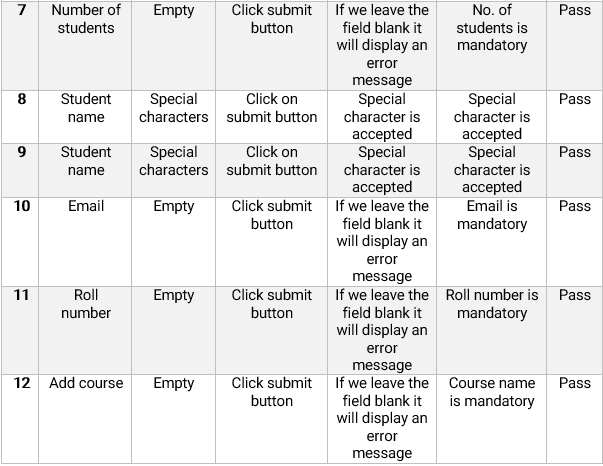
\includegraphics[scale=0.9]{project/images/test2}\hspace*{\fill}
\caption{Test case 2}
\end{figure}

\begin{figure}[H]
\centering
\hfill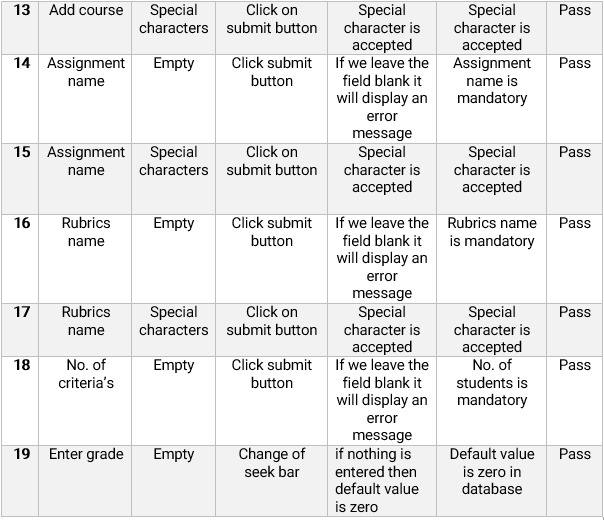
\includegraphics[scale=0.9]{project/images/test3}\hspace*{\fill}
\caption{Test case 3}
\end{figure}
\chapter{Results and Discussion }
During the development of project research was conducted based on similar systems, it was found that none of the systems were developed in a user friendly manner and none of them implemented systems both for android as well as web application.
During the development of the application it was kept in mind that system will be developed both platform android as well as web application.
Creation of rubrics is given as a option to the user to create its own with ease. The user will be entering the criteria based on the assessment and marks will be distributed by the user on each of the criteria.
During the research it was also seen that grading system was not implemented with clarity.Hence that anomaly was taken a account during the development of the project.
Once the assessment of the students are done user will be able to visualize data in graphs as well as they will be able to perform statistical analysis of the data. User will be able to send the assessment to the students via mail.

\chapter{Future Work}
In the future work we are aiming to sync the android application with the web application.
To implement more reliable security features to the online database server.
We will be adding more number of statistical modules to the application. We will also create a student portal wherein the students can submit their assignments.
\chapter{Conclusion }

Rubrics system provides a web-based and mobile-based platform to students as well as the evaluator, where students can upload their work and the evaluator will evaluate their work according to the designed metric developed by the evaluator.This system displays all the performance of the student in a graphical format so that student will get the clear idea about where he/she is good or where he/she is lagging and what is pending jobs and what is completely done.Using Rubric system, the grader can review the student's work as well as give proper feedback to the student and get the personal attention from the grader.
For the best learning as well as evaluation system rubrics system helps teachers and evaluator for the fair evaluation  and communicate with the students personally and provide the proper guidance for better improvement of students.
\newpage
\input{project/appendix.tex}
\appendix
\addcontentsline{toc}{part}{\appendixname}
\newpage
\begin{thebibliography}{99}
\bibitem{RubiStar} RubiStar \url{http://rubistar.4teachers.org/index.php}
"Rubistar Home". Rubistar.4teachers.org. N.p., 2016. Web. 2 Nov. 2016.


\bibitem{Irubric} Irubric
\url{http://www.rcampus.com/indexrubric.cfm}
"Irubric: Home Of Free Rubric Tools: Rcampus". Rcampus.com. N.p., 2016. Web. 2 Nov. 2016.

\bibitem{EssayTagger} EssayTagger
\url{http://www.essaytagger.com/}
"Essaytagger.Com - Transform Assessment, Transform Education". EssayTagger. N.p., 2016. Web. 2 Nov. 2016.


\bibitem{Onlineassessmenttool} Onlineassessmenttool
\url{https://www.onlineassessmenttool.com/}
"Create Assessments For Free". Onlineassessmenttool.com. N.p., 2016. Web. 2 Nov. 2016.


\bibitem{DBIT Moodle} DBIT Moodle 
\url{http://moodle.dbit.in/}
"DBIT Moodle". Moodle.dbit.in. N.p., 2016. Web. 2 Nov. 2016.

\end{thebibliography} % adds the References page
\addcontentsline{toc}{part}{References}
\newpage
\begin{center}
\thispagestyle{empty}
\LARGE{\textbf{Acknowledgements}}\\[1cm]
\end{center}
\linespread{1.13}
\large{\paragraph{}

This project was supported by Don Bosco Institute of Technology. We thank our teachers who provided insight and expertise that greatly assisted the project.\\
We thank Prof. Tayyabali Sayyad for assistance with forming the vision for our project.\\
We would also like to show our gratitude to the IT department teachers for sharing their pearls of wisdom with us during the course of this project. 



\begin{spacing}{0}
\vspace{3.0cm}
%\begin{justify}
\Large{\hfill\textbf{(----------------------------)}\\
\vspace{0.5cm}
\hspace{10.5cm}\textbf{Krupal Jadhav (27)}}\\
%\end{justify}
\end{spacing}
\justify\large{\textbf{Date:}}
 
\printindex
\end{document}
